\section{Stochastic Blockmodels}\label{sec:AdaptedSBMs}

\begin{singlespacing}
    \begin{figure}[H]
    \centering
    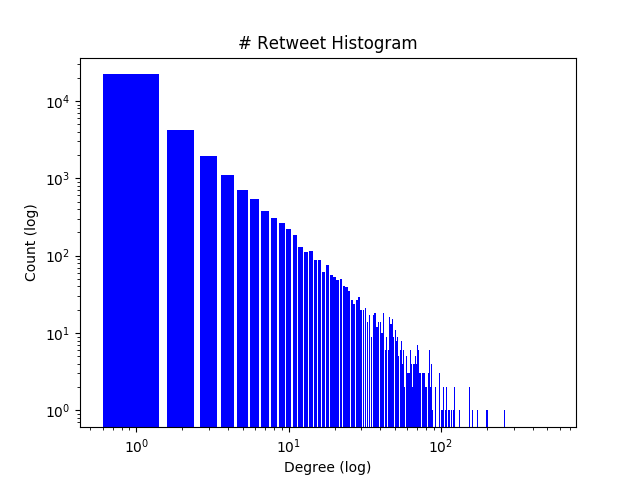
\includegraphics[width=70mm]{Figures/retweet_distribution}
    \caption[Retweet Histogram for Full Political Engagement Graph]{Retweet Histogram for Full Political Engagement Graph}
    \label{fig:retweet_distribution}
    \end{figure}
\end{singlespacing}

As described in section \ref{sec:SBM}, stochastic blockmodels use edge densities
across and within blocks to generate random graph models
\cite{holland1983stochastic}. However, while users may belong to a certain
``party leader block'' or ``topic block''\footnote{In these cases, the blocks
would be users who would only engage with a certain party leader or topic, or
both.} to some degree, these cannot be known a priori and users can be members
of infinite combinations and mixtures of different blocks. As such, a novel
method for generating stochastic blockmodels was developed that approximated
edge densities and is specific to reproducing engagement graphs described in
section \ref{ch:GraphTheory}, where certain users produce objects (tweets,
songs, goods, etc...) and other users choose which ones to engage with. The
algorithm takes in 6 parameters: $n$, $tweet\_dist$, $k$, $m$,
$retweet\_histogram$, $\epsilon$ -- which are described in table
\ref{fig:SBMParameters}.

\begin{singlespacing}
    \begin{center}
    \begin{threeparttable}
    \caption{Adapted Stochastic Blockmodel Parameters}
    \label{fig:SBMParameters}
    \begin{small}
            \begin{tabular}{|l|l|l|}
            \hline
            \textbf{Parameter}              & \textbf{Type}                 & \textbf{Description} \\ \hline
            \emph{n}                        & $Integer$                     & \specialcell{The number of party leader vertices} \\ \hline
            \emph{tweet\_dist}              & $Tuple$                       & \specialcell{A tuple representing a normal distribution \\ $X \sim\mathcal{N}(\mu,\,\sigma^{2})$ that is sampled $n$ times to determine \\ the number of tweet vertices per party leader} \\ \hline
            \emph{$k$}                      & $Integer$                     & The number of topics that a tweet vertex can take on \\ \hline
            \emph{$m$}                      & $Integer$                     & The number of generic user vertices \\ \hline
            \emph{$retweet\_histogram$}     & $Histogram$\tnote{a}          & \specialcell{The distribution of retweets that is sampled $m$ \\ times to get the degree for each generic user} \\ \hline
            \emph{$\epsilon$}               & $Float \in \left[0,1\right]$  & \specialcell{The proportion of the time a generic user will choose \\ the greedy tweet-type\tnote{b}~ rather than choosing based \\ off of the edge probabilities}\\ \hline
            \end{tabular}
    \begin{tablenotes}
        \item[a]    As of March, 2020 -- this took the form as a Numpy histogram:
        a tuple containing the bin boundaries and corresponding densities.    
        \item[b]    For the models generated in this thesis a tweet-type could
        be its topic, the party leader who tweeted it, or its topic \emph{and} the party leader who tweeted it. 
    \end{tablenotes}
        \end{small}
    \end{threeparttable}
    \end{center}
\end{singlespacing}

 The algorithm generates the stochastic block model in three phases. First, all
 the party leader, tweet, and generic user vertices are generated based off of
 $n$, $tweet\_distribution$ and $m$, along with edges between the the party
 leader and tweet vertices. Second, topics are assigned to tweets randomly and
 $m$ samples of the $retweet\_histogram$, shown in figure
 \ref{fig:retweet_distribution}, are generated to determine the retweet degree
 for each user, $D$. Finally, the algorithm loops through each generic user $i$
 and retweets $D_{i}$ tweets. For each retweet user $i$ makes -- edge
 probabilities, $e_{i}$, for each tweet-type are calculated based on the user's
 prior retweet history. The probability of forming an edge between user $i$ and
 a tweet-type $t$, given edge probabilities $e_{i}$, is given by the
 policy\footnote{Policy in this context refers to the probability of choosing an
 action from some set of possible actions and is denoted by $\pi$; all other
 mentions to policy in this thesis refer to categories of messages.} $\pi$ in
 equation \ref{equation:policy_equation}. This is a variation of the
 $\epsilon$-$greedy$ policy, where the tweet-type with the highest probability
 is chosen $\epsilon$ percent of the time, and $(1-\epsilon)$ percent of the
 time tweets are chosen based off of $e_{i}$. After each edge is formed, user
 $i$'s retweet history is updated.

\begin{numcases}{\text{$\pi(t|e_{i})$=}}\label{equation:policy_equation}
    \epsilon                & if $t = argmax_{t}~e_{i}$ \notag \\
    (1-\epsilon)e_{it}    & otherwise \notag
\end{numcases}

While initially the edge probabilities for a user $i$ would be proportional to
their retweet history\footnote{This can be done efficiently by taking the
$softmax$ of the retweet history.}, section \ref{sec:DeepSBMs} demonstrates
how more nuanced edge probabilities can be developed with deep stochastic
blockmodels. The full algorithm is formalized in algorithm \ref{algorithm:SBM}.

\begin{singlespacing}
\begin{algorithm}[H]
    \SetAlgoLined
    \KwResult{A stochastically generated political engagment graph}
    initialize $G$ as an empty graph\;
    initialize $T$ as an array of all different tweet-types\;
    initialize $n$ party leader vertices in $G$\;
    initialize $m$ generic user vertices in $G$\;
    \For{$i\leftarrow 1$ \KwTo $n$}{
        initialize $X \sim\mathcal{N}(\mu,\,\sigma^{2})$ tweet vertices in $G$\;
        assign tweet vertices random topics from $[1,...,k]$\;
        add edges from tweet vertices to party leader $i$\;
    }
    generate retweet degree array $D$ of size $m$ by sampling $retweet\_histogram$\;
    \For{$i\leftarrow 1$ \KwTo $m$}{
        initialize $user\_history$ array of size $|T|$ with all 0s\;
        \For{$j\leftarrow 1$ \KwTo $D_{i}$}{
            generate edge probabilities $e_{i}$\;
            add an edge from user $i$ to a tweet of tweet-type $t$ based on $\pi(t|e_{i})$\;
            $user\_history_{t}+=1$
        } 
     }
     \KwRet{$G$}
     \caption{Stochastic blockmodel for modelling political engagement}
     \label{algorithm:SBM}
\end{algorithm}
\end{singlespacing}


\subsubsection{Deep Stochastic Blockmodels for Modelling Political Engagement}\label{sec:DeepSBMs}

As discussed in section \ref{sec:AdaptedSBMs}, the edge probabilities for a user
retweeting a tweet-type can be calculated in various ways. A further nuance that
can be added is incorporating real world data into the edge probability
calculation. Data used to generate the complete political engagement graph in
figure \ref{fig:og_graph} was used to train two feed-forward artificial neural
networks (ANN) to aid in the edge probability calculation: one that predicts the
next party leader a user would tweet given the prior party leaders they had
retweeted, and one that predicts which topic a user would retweet given the
previous topics of tweets that user had retweeted. Figure
\ref{fig:confusion_matrices} shows the confusion matrices for these two ANNs.
Both ANNs are standard feed forward neural networks with two dense layers
containing 32 and 16 nodes respectively. Each attained between 85-87\% accuracy.

\begin{singlespacing}
    \begin{figure}
        \centering
        \begin{tabular}{cc}
          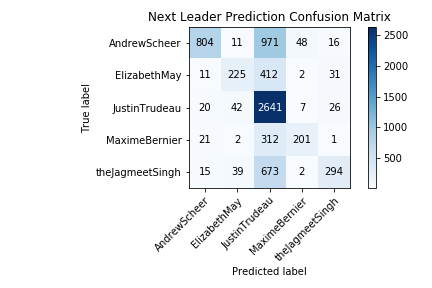
\includegraphics[width=60mm]{Figures/next_leader_CM}
          &
          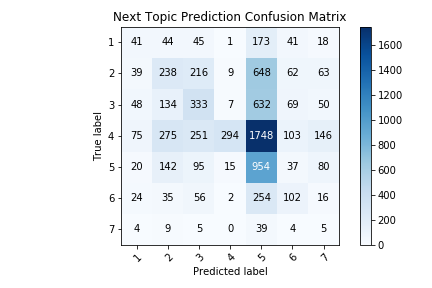
\includegraphics[width=60mm]{Figures/next_topic_CM}
          \\
        (a) ``Next Leader'' Confusion Matrix & (b) ``Next Topic'' Confusion Matrix \\[6pt]
        \end{tabular}
        \caption[ANN Confusion Matrices]{ANN Confusion Matrices}
        \label{fig:confusion_matrices}
    \end{figure}
\end{singlespacing}

Sections \ref{sec:SPLBM}, \ref{sec:STBM} and \ref{sec:SHBM} will demonstrate
both the utility of these ANNs in generating the stochastic blockmodels in
comparison to the standard edge probability calculation.

\subsection{Stochastic Party Leader Blockmodel}\label{sec:SPLBM}

The stochastic party leader blockmodel generates user behaviour only taking into
account the previous party leaders each user had engaged with prior. The
tweet-types therefore are all the different party leaders that could be
retweeted and $e_{i}$ represents the weights of retweeting each party leader.
For each user, when deciding which tweet they are to retweet, their retweet
history is converted into a probability distribution (ex.\
$user\_history_{i}=[JT=0,AS=1,JS=3,EM=2,MB=0]$ generates
$e_{i}=[JT=0.09,AS=0.19,JS=0.36,EM=0.27,MB=0.09]$). In this sense, it models a
world in which politically engaged Twitter users only engage along the axis of
party leaders, with a complete disregard for the topics tweeted about. Figure
\ref{fig:stochastic_party_leader_model} shows two examples of stochastic party
leader blockmodels: one in which edge probabilities are proportional to the
number of times that user's retweeted each party leader, and one in which edge
probabilities are determined with the ANN described in section
\ref{sec:DeepSBMs}.

\begin{singlespacing}
    \begin{figure}
        \centering
        \begin{tabular}{cc}
          \includegraphics[width=0.40\textwidth]{Figures/simple_stochastic_party_leader_model}
          &
          \includegraphics[width=0.40\textwidth]{Figures/ann_stochastic_party_leader_model}
          \\
        (a) Stochastic Party Leader Blockmodel & (b) ANN Adaption\\[6pt]
        \end{tabular}
        \caption[Stochastic Party Leader Blockmodels]{Stochastic Party Leader Blockmodels}
        \label{fig:stochastic_party_leader_model}
    \end{figure}
\end{singlespacing}

\subsection{Stochastic Topic Blockmodel}\label{sec:STBM}

Conversely, the stochastic topic blockmodel models a world in which politically
engaged Twitter users only engage along the axis of topics. In this case, the
tweet-types are the various different topics that a user can engage with. Here,
the tweet-type history of a user is converted into a probability distribution,
and with a probability of $\epsilon$, that user will retweet any tweet with the
topic that has the highest activation -- regardless of which party leader
tweeted it. Figure \ref{fig:stochastic_topic_model} shows two examples of
stochastic topic blockmodels: one in which edge probabilities are proportional
to a user's topic retweet history, and one in which edge probabilities are
determined with the ANN described in section \ref{sec:DeepSBMs}.

\begin{singlespacing}
    \begin{figure}
        \centering
        \begin{tabular}{cc}
          \includegraphics[width=0.40\textwidth]{Figures/simple_stochastic_topic_model} &
          \includegraphics[width=0.40\textwidth]{Figures/ann_stochastic_topic_model} \\
        (a) Stochastic Topic Blockmodel & (b) ANN Adaption\\[6pt]
        \end{tabular}
        \caption[Stochastic Topic Blockmodels]{Stochastic Topic Blockmodels}
        \label{fig:stochastic_topic_model}
    \end{figure}
\end{singlespacing}

\subsection{Stochastic Hybrid Blockmodel}\label{sec:SHBM}

The final model developed is a hybrid of the stochastic party leader blockmodel,
and the stochastic topic blockmodel. Here, two history vectors for each user are
captured -- the $n$ dimensional party leader history vector, and the $k$
dimensional topic history vector. After each respective vector is converted into
a probability distribution, the edge probability of topic $t$ by party leader
$p$ is determined by some constant $\alpha$\footnote{This has no relation to the
LDA parameter $\alpha$ referred to in section \ref{sec:LDA}} and the function:

\begin{equation}
    edge\_probability(party leader=p, topic=t)=\alpha P(p)+(1-\alpha)P(t)
\end{equation}

Where $P(p)$ is index $p$ of that user's \emph{party leader} probability
distribution, $P(t)$ is index $t$ of that user's \emph{topic} probability
distribution, and $\alpha$ is some constant that determines the relative
weighting of the two. As $\alpha$ approaches $1$, the hybrid model becomes
equivalent to the stochastic party leader blockmodel -- and as $\alpha$
approaches $0$ the model approaches the stochastic topic blockmodel. This model
then generates different ``worlds'' in which users' political engagement falls
on the spectrum from only caring about \emph{party leaders} to only caring about
\emph{topics}.

\begin{singlespacing}
    \begin{figure}
        \centering
        \begin{tabular}{cc}
          \includegraphics[width=0.40\textwidth]{Figures/standard_SHBm_ex} &
          \includegraphics[width=0.40\textwidth]{Figures/deep_SHBm_ex} \\
        (a) Standard SHBm ($\alpha$=0.60) & (b) Deep SHBm ($\alpha$=0.60)\\[6pt]
        \end{tabular}
        \caption[Stochastic Topic Blockmodels]{Stochastic Topic Blockmodels}
        \label{fig:SHBm_examples}
    \end{figure}
\end{singlespacing}

\subsection{NetLSD for Describing Political Engagement}\label{sec:NetLSDForSBM}

The final objective of comparing the relative importance of topics and party
leaders in driving political engagement requires comparing the structure of
target graph shown in section \ref{ch:GraphTheory}, and various hybrid models
generated with different values of $\alpha$. Using the Network Laplacian
Spectral Descriptor (NetLSD) described in section \ref{sec:NetLSD} by Tsitsulin
et al. the optimal $\alpha$ value can be determined in a scale-adaptive,
size-invariant, and permutation-invariant manner \cite{netlsd}.

Given the $O(n^{3})$ complexity involved in calculating the eigenvalues of a
graphs normalized Laplacian matrix it is advantageous to generate sufficiently
small hybrid models when fitting them to the original engagement graph (see
figure \ref{fig:og_graph}). To determine how large a graph of this nature needs
to be to capture its underlying structure -- tweets of the original graph were
sampled, keeping all the retweet edges, and then compared to the heat trace
signature of the original graph. This is shown graphically in figure
\ref{fig:dist_from_original_graph_over_sample_size}, the x-axis represents how
many tweets \emph{per party leader} were sampled from the original graph and the
y-axis represents the $L_{2}$ distance from the original engagement graph's heat
trace signature. 

\begin{singlespacing}
    \begin{figure}[H]
    \centering
    \begin{tabular}{cc}
        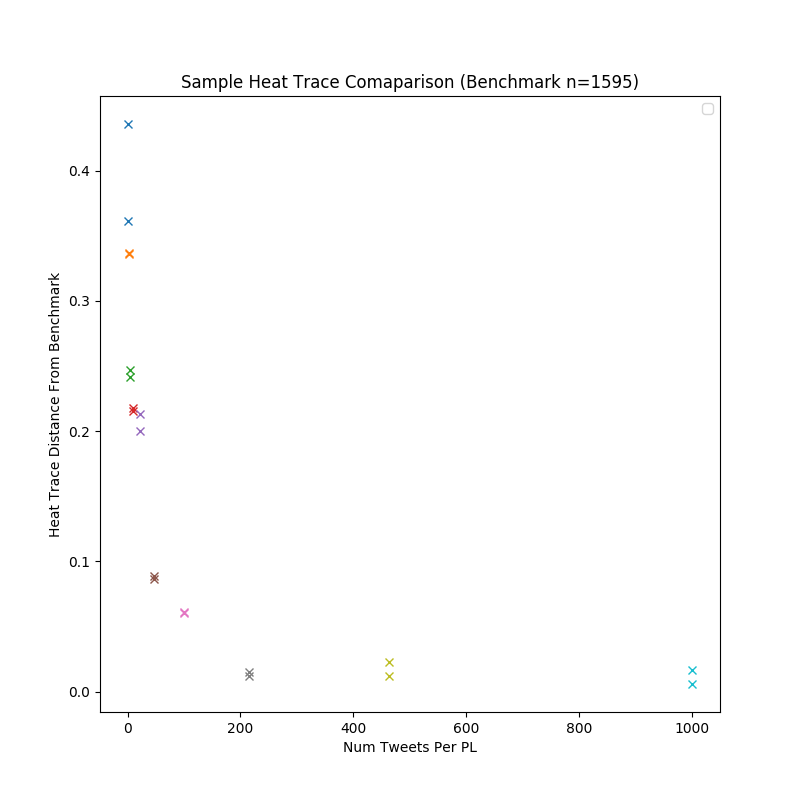
\includegraphics[width=0.40\textwidth]{Figures/dist_from_original_graph_over_sample_size} &
        \includegraphics[width=0.40\textwidth]{Figures/sampled_graph} \\
        (a) Heat Trace Signature Distances & (b) Engagement Graph (215 Tweets per PL)\\[6pt]
    \end{tabular}
    \caption[Heat Trace Signature Distance as a Function of Graph Sample Size]{Heat Trace Signature Distance as a Function of Graph Sample Size}
    \label{fig:dist_from_original_graph_over_sample_size}
    \end{figure}
\end{singlespacing}

As can be seen from figure \ref{fig:dist_from_original_graph_over_sample_size},
there are diminishing returns for graphs with more than 215 tweets per party
leader. Therefore, for each of the party leader vertices generated with the
hybrid models -- each one generated a number of tweets by a random variable $X$
that is distributed normally where $X \sim
\mathcal{N}(\mu=215,\,\sigma^{2}=70)$.

\subsection{Results}\label{sec:SBMsResults}

The stochastic hybrid blockmodel (SHBm) gives the ability to define different
``worlds'' in which policy and party leaders drive engagement to different
degrees. NetLSD gives the ability to compare the structural similarity of graphs
in a scale-adaptive, size-invariant, and permutation-invariant manner. By
performing a sweep of different $\alpha$ values for the hybrid models, and
measuring which one produces the heat trace signature with the smallest $L_2$
distance to the original graph, the final objective of putting Ezra Klein's
hypothesis to task can be achieved. All graphs were generated with $n=5$, $k=7$,
$tweet\_dist=(\mu=215,\,\sigma^{2}=70)$, $m=8826$, $retweet\_histogram$ derived
from the original engagement graph, and $\epsilon=0.95$. $\alpha$ values ranging
between 0 and 1, with increments of 0.05 were used to generate the different
hybrid models. Four models were generated per $\alpha$ and the mean distance was
used to determine the final distance.

The results of this experiment are striking: in both the deep SHBm, which uses
the ANN to calculate edge probabilities, and the standard SHBm, which makes edge
probabilities proportional to the user's retweet history, it is clear that both
\emph{what} the message is and \emph{who} tweeted the message drive political
engagement. The standard SHBm shows a clear trend where $\alpha$ values that
privilege policy over party leader, or vice versa, have a further distance from
original engagement graph than ones that blend the two. These hybrid models had
the best fit when $\alpha=0.6$. The deep SHBm had an optimal fit when
$\alpha=0.4$. The full tabular data is shown in table
\ref{fig:tab_SHBm_results}, and the results are visualized in figure
\ref{fig:SHBm_results}.

\begin{singlespacing}
    \begin{figure}
        \centering
        \begin{tabular}{cc}
            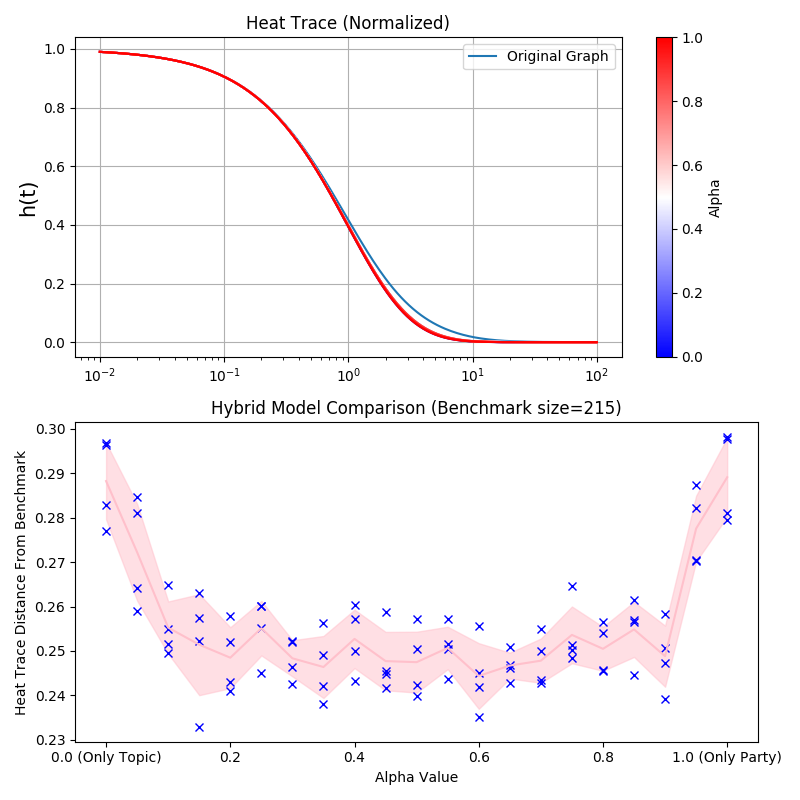
\includegraphics[width=0.40\textwidth]{Figures/standard_heat_trace_plot} &
            \includegraphics[width=0.40\textwidth]{Figures/ann_heat_trace_plot} \\
            (a) Standard SHBm $L_{2}$ Plots & (b) Deep SHBm $L_{2}$ Plots\\[6pt]
        \end{tabular}
        \caption[Stochastic Topic Blockmodels]{Stochastic Topic Blockmodels}
        \label{fig:SHBm_results}
    \end{figure}
\end{singlespacing}

\begin{singlespacing}
    \begin{center}
    \begin{threeparttable}
    \caption{Results of NetLSD Comparison of SHBm Models}
    \label{fig:tab_SHBm_results}\begin{small}
        \begin{tabular}{|l|c|c|c|c|c|c|c|} \hline
        \multicolumn{1}{|c|}{} & \multicolumn{3}{|c|}{Standard SHBm} & \multicolumn{3}{|c|}{Deep SHBm} \\ \hline
        \multicolumn{1}{|c|}{$\alpha$} & Min $L_{2}$ & Mean $L_{2}$ & $\sigma^{2}$  & Min $L_{2}$ &  Mean $L_{2}$ & $\sigma^{2}$ \\  \cline{6-7}
        \hline
            0.00  & 0.2648 & 0.2756 & 0.0083   &  0.2173 & 0.2276 & 0.0062 \\
        \hline
            0.05  & 0.2475 & 0.2603 & 0.0104   &  0.2111 & 0.2201 & 0.0073 \\
        \hline
            0.10  & 0.2385 & 0.2440 & 0.0057   &  0.2030 & 0.2231 & 0.0117 \\
        \hline
            0.15  & \textbf{0.2225} & 0.2403 & 0.0109   &  0.2176 & 0.2217 & 0.0061 \\
        \hline
            0.20  & 0.2303 & 0.2375 & 0.0066   &  0.2210 & 0.2260 & 0.0037 \\
        \hline
            0.25  & 0.2343 & 0.2439 & 0.0059   &  0.2172 & 0.2241 & 0.0067 \\
        \hline
            0.30  & 0.2319 & 0.2374 & 0.0039   &  0.2207 & 0.2260 & 0.0058 \\
        \hline
            0.35  & 0.2274 & 0.2355 & 0.0067   &  \textbf{0.2022} & 0.2174 & 0.0095 \\
        \hline
            0.40  & 0.2328 & 0.2418 & 0.0063   &  0.2096 & \textbf{0.2134} & 0.0031 \\
        \hline
            0.45  & 0.2313 & 0.2370 & 0.0063   &  0.2181 & 0.2257 & 0.0067 \\
        \hline
            0.50  & 0.2296 & 0.2368 & 0.0066   &  0.2255 & 0.2355 & 0.0085 \\
        \hline
            0.55  & 0.2329 & 0.2396 & 0.0046   &  0.2440 & 0.2565 & 0.0116 \\
        \hline
            0.60  & 0.2246 & \textbf{0.2336} & 0.0071   &  0.2249 & 0.2508 & 0.0187 \\
        \hline
            0.65  & 0.2320 & 0.2358 & 0.0028   &  0.2260 & 0.2418 & 0.0125 \\
        \hline
            0.70  & 0.2320 & 0.2369 & 0.0048   &  0.2260 & 0.2418 & 0.0125 \\
        \hline
            0.75  & 0.2374 & 0.2425 & 0.0061   &  0.2610 & 0.2718 & 0.0079 \\
        \hline
            0.80  & 0.2347 & 0.2394 & 0.0047   &  0.2603 & 0.2692 & 0.0062 \\
        \hline
            0.85  & 0.2338 & 0.2436 & 0.0060   &  0.2484 & 0.2597 & 0.0081 \\
        \hline
            0.90  & 0.2286 & 0.2378 & 0.0066   &  0.2604 & 0.2684 & 0.0058 \\
        \hline
            0.95  & 0.2584 & 0.2654 & 0.0071   &  0.2432 & 0.2581 & 0.0111 \\
        \hline
            1.00  & 0.2672 & 0.2765 & 0.0085   &  0.2506 & 0.2611 & 0.0098 \\
        \hline
        \end{tabular}
    \end{small}
    \end{threeparttable}
\end{center}
\end{singlespacing}
